% ─────────────────────────────────────────────────────────────────────────────
% RFEM vs Sink-Aware RFEM — Visual Comparison Report
% Mohsin Imam & Gourab Roy  |  TRDP-1  |  IPCV/UAM  |  2026
% ─────────────────────────────────────────────────────────────────────────────
\documentclass[a4paper,11pt]{article}

\usepackage[margin=1.8cm]{geometry}
\usepackage{graphicx}
\usepackage{amsmath}
\usepackage{amssymb}
\usepackage{caption}
\usepackage{subcaption}
\usepackage{xcolor}
\usepackage{titlesec}
\usepackage{parskip}
\usepackage{microtype}
\usepackage{hyperref}
\usepackage{tcolorbox}
\usepackage{float}
\usepackage{booktabs}

\captionsetup{font=small, labelfont=bf, labelsep=period,
              justification=centering, skip=4pt}
\captionsetup[subfigure]{font=footnotesize, labelfont=bf, skip=2pt}

\definecolor{bertblue}{RGB}{31,73,125}
\definecolor{cliptextgreen}{RGB}{0,110,60}
\definecolor{clipvisionred}{RGB}{140,30,30}
\definecolor{formulabg}{RGB}{245,248,255}
\definecolor{sinkred}{RGB}{180,30,30}

\titleformat{\section}{\large\bfseries\color{bertblue}}{}{0em}{}[\titlerule]
\titleformat{\subsection}{\normalsize\bfseries}{}{0em}{}

\setlength{\parskip}{4pt}
\setlength{\parindent}{0pt}

\newcommand{\BERT}{figs_pdf/S1}
\newcommand{\BERTsa}{figs_bert_sink_aware/S1}
\newcommand{\CLIPTxt}{figs_clip_text_sink_aware/S1}
\newcommand{\CLIPVstd}{figs_pdf_clip_vision/I1}
\newcommand{\CLIPVsa}{figs_clip_vision_sink_aware/I1}

% ─────────────────────────────────────────────────────────────────────────────
\begin{document}

{\centering
  \Large\bfseries RFEM: Standard vs.\ Sink-Aware\\[6pt]
  \normalsize Mohsin Imam \& Gourab Roy \quad|\quad TRDP-1 \quad|\quad IPCV/UAM \quad|\quad 2026\\[2pt]
  \small Supervisors: Prof.\ Jenny Benois-Pineau \quad Marcos Escudero-Vi\~{n}olo\\[4pt]
}
\noindent\rule{\linewidth}{0.8pt}

% =============================================================================
\section*{Methodology}
% =============================================================================

\textbf{Standard RFEM — four stages:}

\medskip
\textbf{Stage A — Per-head rollout.}\\
Each attention head $h$ is rolled out separately across all $L$ layers. Rows are re-normalised after adding the identity:
\[
  \hat{A}_h = \prod_{l=1}^{L}\!\bigl(A_h^{(l)} + I\bigr)
\]

\medskip
\textbf{Stage B — K-$\sigma$ filter.}\\
Entries below the per-head threshold are zeroed out:
\[
  \tilde{A}_h(i,j) = \begin{cases} \hat{A}_h(i,j), & \hat{A}_h(i,j) \geq \mu_h + K\sigma_h \\ 0, & \text{otherwise} \end{cases}
\]
where $\mu_h$ and $\sigma_h$ are computed from the read-out row of $\hat{A}_h$.

\medskip
\textbf{Stage C — Weighted head aggregation.}\\
Filtered per-head masks are combined using the per-head maximum as weight:
\[
  A_{\mathrm{rfem}} = \sum_{h=1}^{H} w_h\,\tilde{A}_h, \qquad w_h = \max(\hat{A}_h)
\]

\medskip
\textbf{Stage D — Read-out.}\\
Importance scores are extracted from the read-out row of $A_{\mathrm{rfem}}$:
BERT $\to$ \texttt{[CLS]} row $\to$ token bars;\quad
CLIP-Text $\to$ \texttt{[EOS]} row $\to$ token bars;\quad
CLIP-Vision $\to$ \texttt{[CLS]} row $\to$ $7{\times}7$ patch heatmap.

\bigskip
\textbf{Sink-aware variant:}

\medskip
\textbf{Problem.}\\
Certain structural tokens act as \emph{attention sinks} — they absorb disproportionate probability mass: \texttt{[CLS]}/\texttt{[SEP]} in BERT, BOS/EOS in CLIP-Text, and the CLS-self position in CLIP-Vision. Sink entries inflate $\sigma_h$, pushing the threshold above all content tokens and zeroing them out.

\medskip
\textbf{Fix.}\\
$\mu_h$ and $\sigma_h$ are computed from the read-out row \emph{excluding the sink token columns}. The threshold is then calibrated to the content-token distribution only, so content tokens are no longer suppressed.

\clearpage
% =============================================================================
\section{\textcolor{bertblue}{BERT — Sentence S1}}
% =============================================================================

\subsection*{Baseline: Vanilla Attention}

\begin{figure}[H]
  \centering
  \begin{subfigure}[t]{0.48\linewidth}
    
\includegraphics[width=\linewidth]{\BERT/S1_M1_vanilla_matrix.pdf}
    \caption{Last-layer mean attention matrix (all 12 heads averaged). \texttt{[CLS]} and \texttt{[SEP]} columns attract the dominant mass.}
  \end{subfigure}\hfill
  \begin{subfigure}[t]{0.48\linewidth}
    
\includegraphics[width=\linewidth]{\BERT/S1_M1_vanilla_cls_bar.pdf}
    \caption{Vanilla CLS read-out scores. Sink tokens \texttt{[CLS]} and \texttt{[SEP]} dominate; all content words are suppressed.}
  \end{subfigure}
  \caption{\textbf{Vanilla attention (BERT, S1).} Raw last-layer attention already shows severe sink behaviour before any rollout or filtering.}
\end{figure}

\begin{figure}[H]
  \centering
  
\includegraphics[width=\linewidth]{\BERT/S1_M2_rollout_cls_bar.pdf}
  \caption{\textbf{Standard attention rollout — CLS row scores (BERT, S1).} Multiplicative rollout across all 12 layers amplifies the sink effect: \texttt{[CLS]} and \texttt{[SEP]} absorb virtually all weight, leaving content tokens near zero.}
\end{figure}

% ─────────────────────────────────────────────────────────────────────────────
\subsection*{RFEM — Stage A: Per-Head Rollout}

\begin{figure}[H]
  \centering
  \begin{subfigure}[t]{0.48\linewidth}
    
\includegraphics[width=\linewidth]{\BERT/S1_M3_step1_head01_matrix.pdf}
    \caption{Head 1 rolled-out matrix $\hat{A}_{h=1}$. The \texttt{[CLS]} column (leftmost) is the dominant sink.}
  \end{subfigure}\hfill
  \begin{subfigure}[t]{0.48\linewidth}
    
\includegraphics[width=\linewidth]{\BERT/S1_M3_step1_head12_matrix.pdf}
    \caption{Head 12 rolled-out matrix $\hat{A}_{h=12}$. Both \texttt{[CLS]} and \texttt{[SEP]} columns concentrate the weight.}
  \end{subfigure}
  \caption{\textbf{Per-head rollout matrices (BERT, S1).} Every head independently accumulates sink mass through all 12 layers. The K-$\sigma$ filter must overcome this inflated baseline to surface content tokens.}
\end{figure}

% ─────────────────────────────────────────────────────────────────────────────
\subsection*{RFEM — Stage C: Weighted Head Aggregation}

\begin{figure}[H]
  \centering
  \begin{subfigure}[t]{0.48\linewidth}
    
\includegraphics[width=\linewidth]{\BERT/S1_M3_step3_agg_weighted_K0.5.pdf}
    \caption{Standard RFEM $A_\mathrm{rfem}$ ($K{=}0.5$). Sink columns still carry dominant weight after filtering.}
  \end{subfigure}\hfill
  \begin{subfigure}[t]{0.48\linewidth}
    
\includegraphics[width=\linewidth]{\BERTsa/S1_M3_step3_agg_weighted_K0.5.pdf}
    \caption{SA-RFEM $A_\mathrm{rfem}$ ($K{=}0.5$). Sink columns suppressed; content token columns are recovered.}
  \end{subfigure}
  \caption{\textbf{Weighted aggregation matrix — Standard vs.\ Sink-Aware RFEM at $K{=}0.5$ (BERT, S1).} In the sink-aware variant, $\mu_h$ and $\sigma_h$ are estimated from content-only CLS row entries, making the threshold meaningful for content tokens.}
\end{figure}

% ─────────────────────────────────────────────────────────────────────────────
\subsection*{RFEM — Stage D: Token Importance Scores (Standard RFEM)}

\begin{figure}[H]
  \centering
  \begin{subfigure}[t]{0.235\linewidth}
    
\includegraphics[width=\linewidth]{\BERT/S1_M4_rfem_filtered_cls_bar_K0.0.pdf}
    \caption{Standard RFEM\\$K{=}0.0$}
  \end{subfigure}\hfill
  \begin{subfigure}[t]{0.235\linewidth}
    
\includegraphics[width=\linewidth]{\BERT/S1_M4_rfem_filtered_cls_bar_K0.3.pdf}
    \caption{Standard RFEM\\$K{=}0.3$}
  \end{subfigure}\hfill
  \begin{subfigure}[t]{0.235\linewidth}
    
\includegraphics[width=\linewidth]{\BERT/S1_M4_rfem_filtered_cls_bar_K0.5.pdf}
    \caption{Standard RFEM\\$K{=}0.5$}
  \end{subfigure}\hfill
  \begin{subfigure}[t]{0.235\linewidth}
    
\includegraphics[width=\linewidth]{\BERT/S1_M4_rfem_filtered_cls_bar_K1.0.pdf}
    \caption{Standard RFEM\\$K{=}1.0$}
  \end{subfigure}
  \caption{\textbf{Standard RFEM — CLS token scores for all K values (BERT, S1).} \texttt{[CLS]}/\texttt{[SEP]} sink tokens retain high scores at every threshold level. Increasing $K$ aggressively zeros out content tokens rather than filtering the sinks.}
\end{figure}

% ─────────────────────────────────────────────────────────────────────────────
\subsection*{RFEM — Stage D: Token Importance Scores (Sink-Aware RFEM)}

\begin{figure}[H]
  \centering
  
\includegraphics[width=\linewidth]{\BERTsa/S1_M3_step4_K_sweep_importance.pdf}
  \caption{\textbf{Sink-Aware RFEM — CLS token importance across all K values (BERT, S1).} With sink columns excluded from threshold estimation, content words such as \textit{beautiful}, \textit{resilience}, and \textit{portrait} surface with meaningful raw scores. Higher $K$ progressively removes low-confidence tokens while the most salient content words remain stable.}
\end{figure}

\clearpage
% =============================================================================
\section{\textcolor{cliptextgreen}{CLIP-Text Encoder — Sentence S1}}
% =============================================================================

\subsection*{Baseline: Vanilla Attention}

\begin{figure}[H]
  \centering
  \begin{subfigure}[t]{0.48\linewidth}
    
\includegraphics[width=\linewidth]{\CLIPTxt/S1_M1_vanilla_matrix.pdf}
    \caption{Last-layer mean attention matrix. The BOS column (far left) and EOS diagonal entry absorb the dominant mass in every row.}
  \end{subfigure}\hfill
  \begin{subfigure}[t]{0.48\linewidth}
    
\includegraphics[width=\linewidth]{\CLIPTxt/S1_M1_vanilla_eos_bar.pdf}
    \caption{Vanilla EOS read-out scores. BOS and EOS tokens monopolise the read-out row; content tokens are negligible.}
  \end{subfigure}
  \caption{\textbf{Vanilla attention (CLIP-Text, S1).} Causal masking concentrates the EOS row on BOS — the structural sink — before any RFEM processing.}
\end{figure}

\begin{figure}[H]
  \centering
  
\includegraphics[width=\linewidth]{\CLIPTxt/S1_M2_rollout_eos_bar.pdf}
  \caption{\textbf{Standard attention rollout — EOS row scores (CLIP-Text, S1).} Layer-by-layer rollout amplifies BOS sink dominance. Content tokens are entirely suppressed, making standard rollout uninformative for text interpretation.}
\end{figure}

% ─────────────────────────────────────────────────────────────────────────────
\subsection*{RFEM — Stage A: Per-Head Rollout}

\begin{figure}[H]
  \centering
  \begin{subfigure}[t]{0.48\linewidth}
    
\includegraphics[width=\linewidth]{\CLIPTxt/S1_M3_step1_head01_matrix.pdf}
    \caption{Head 1 rolled-out matrix $\hat{A}_{h=1}$. BOS column (col 0) concentrates the largest weight mass.}
  \end{subfigure}\hfill
  \begin{subfigure}[t]{0.48\linewidth}
    
\includegraphics[width=\linewidth]{\CLIPTxt/S1_M3_step1_head08_matrix.pdf}
    \caption{Head 8 rolled-out matrix $\hat{A}_{h=8}$. Both BOS and EOS positions act as sinks in this head.}
  \end{subfigure}
  \caption{\textbf{Per-head rollout matrices (CLIP-Text, S1).} All 8 heads exhibit BOS-dominated columns after full rollout. The inflated $\sigma_h$ in standard RFEM prevents content tokens from surviving the K-$\sigma$ filter.}
\end{figure}

% ─────────────────────────────────────────────────────────────────────────────
\subsection*{RFEM — Stage C: Weighted Head Aggregation}

\begin{figure}[H]
  \centering
  \begin{subfigure}[t]{0.48\linewidth}
    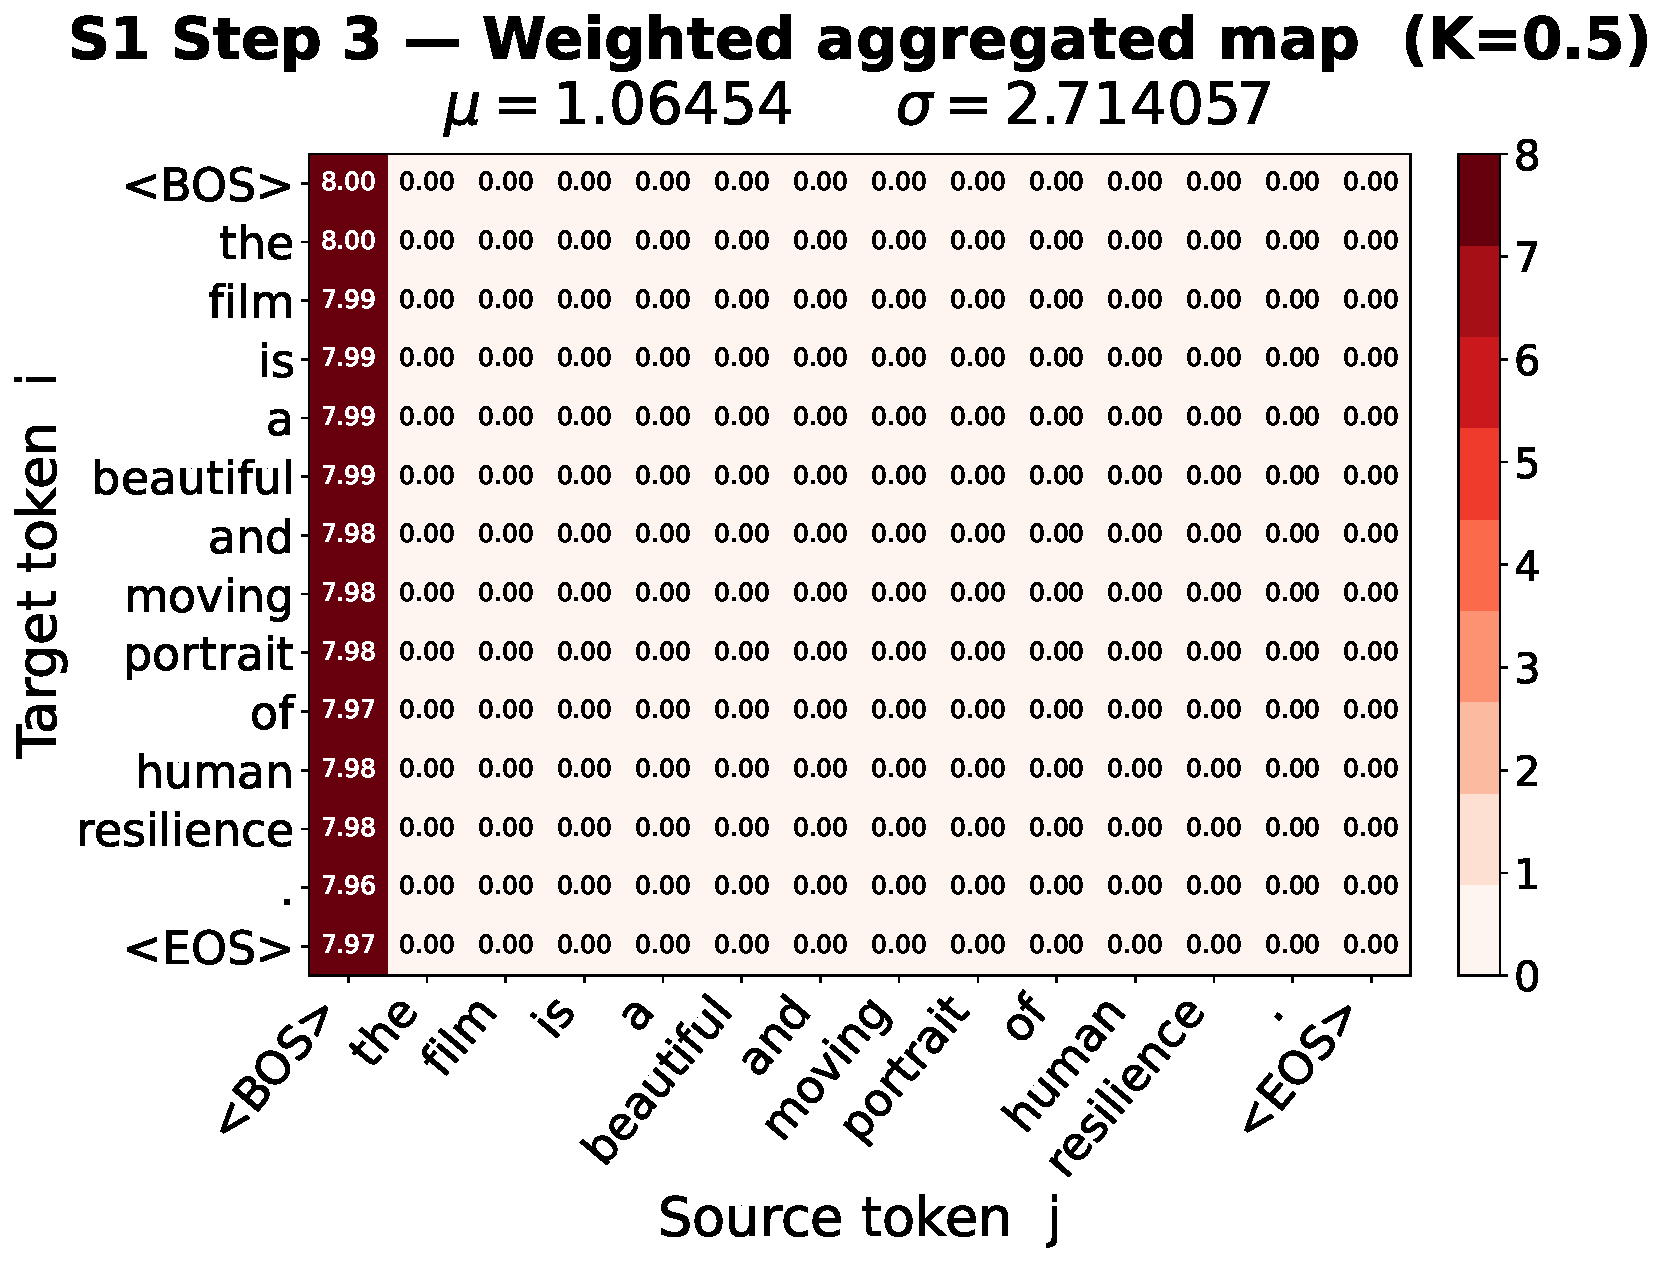
\includegraphics[width=\linewidth]{figs_pdf_clip/S1/S1_M3_step3_agg_weighted_K0.5.pdf}
    \caption{Standard RFEM $A_\mathrm{rfem}$ ($K{=}0.5$). BOS column still dominates; content columns are near-zero.}
  \end{subfigure}\hfill
  \begin{subfigure}[t]{0.48\linewidth}
    
\includegraphics[width=\linewidth]{\CLIPTxt/S1_M3_step3_agg_weighted_K0.5.pdf}
    \caption{SA-RFEM $A_\mathrm{rfem}$ ($K{=}0.5$). BOS/EOS excluded from threshold — content columns become visible.}
  \end{subfigure}
  \caption{\textbf{Weighted aggregation matrix — Standard vs.\ Sink-Aware RFEM at $K{=}0.5$ (CLIP-Text, S1).} The sink-aware threshold is calibrated against content-token values in the EOS row only, enabling content signal to propagate through the filter.}
\end{figure}

% ─────────────────────────────────────────────────────────────────────────────
\subsection*{RFEM — Stage D: Token Importance Scores (Standard RFEM)}

\begin{figure}[H]
  \centering
  \begin{subfigure}[t]{0.235\linewidth}
    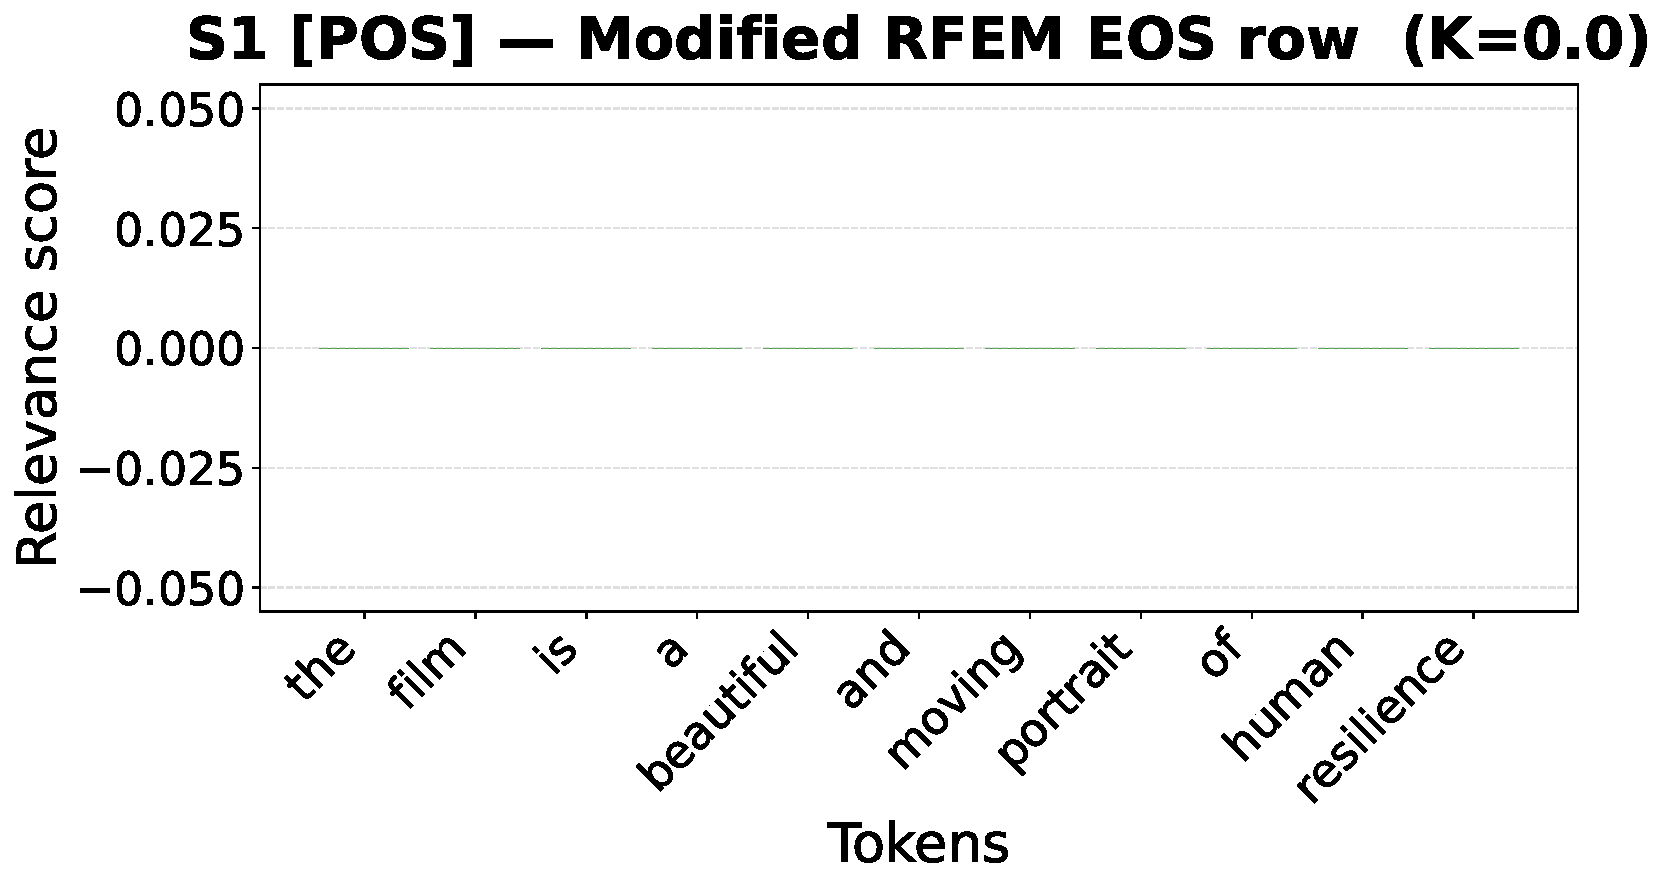
\includegraphics[width=\linewidth]{figs_pdf_clip/S1/S1_M4_rfem_filtered_eos_bar_K0.0.pdf}
    \caption{Standard RFEM\\$K{=}0.0$}
  \end{subfigure}\hfill
  \begin{subfigure}[t]{0.235\linewidth}
    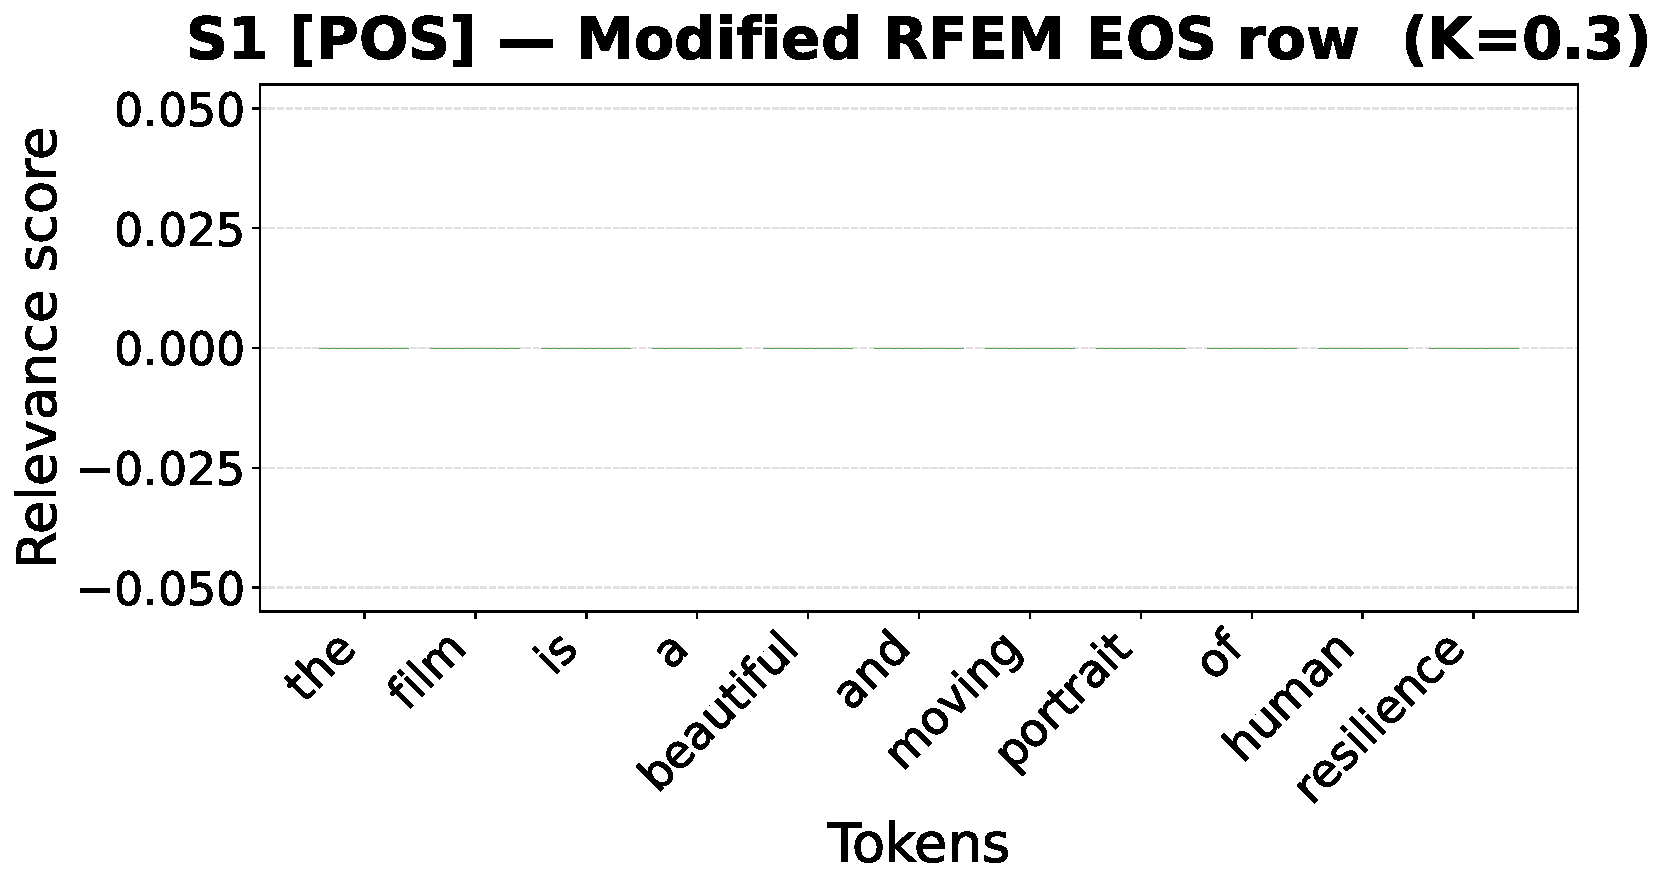
\includegraphics[width=\linewidth]{figs_pdf_clip/S1/S1_M4_rfem_filtered_eos_bar_K0.3.pdf}
    \caption{Standard RFEM\\$K{=}0.3$}
  \end{subfigure}\hfill
  \begin{subfigure}[t]{0.235\linewidth}
    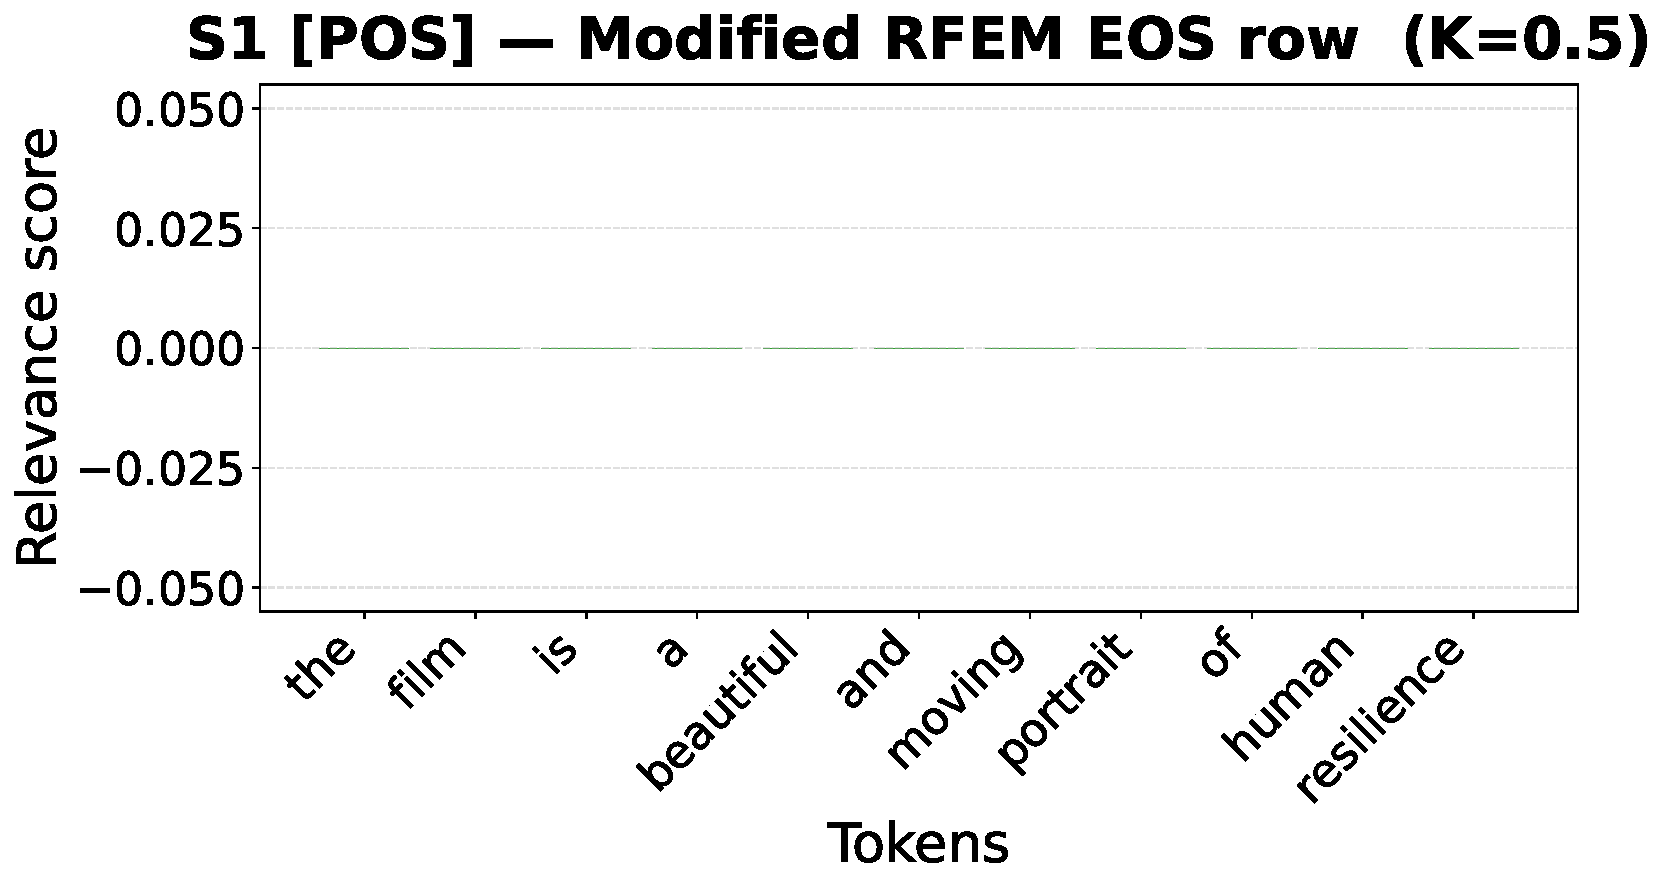
\includegraphics[width=\linewidth]{figs_pdf_clip/S1/S1_M4_rfem_filtered_eos_bar_K0.5.pdf}
    \caption{Standard RFEM\\$K{=}0.5$}
  \end{subfigure}\hfill
  \begin{subfigure}[t]{0.235\linewidth}
    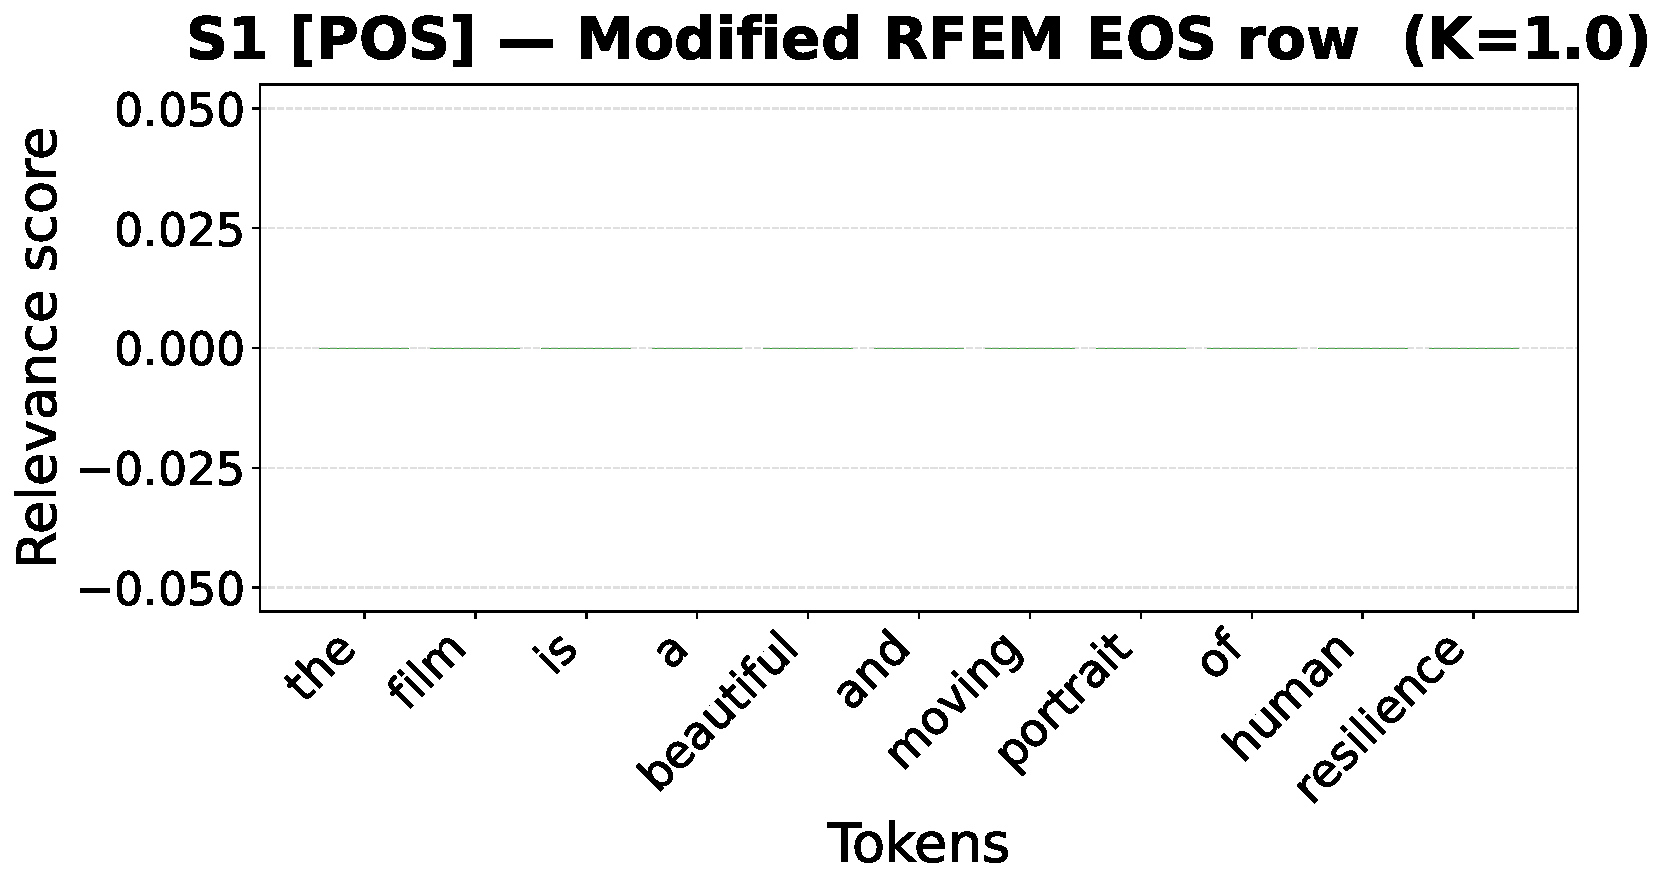
\includegraphics[width=\linewidth]{figs_pdf_clip/S1/S1_M4_rfem_filtered_eos_bar_K1.0.pdf}
    \caption{Standard RFEM\\$K{=}1.0$}
  \end{subfigure}
  \caption{\textbf{Standard RFEM — EOS token scores for all K values (CLIP-Text, S1).} All content tokens score zero at every threshold because the BOS sink inflates $\sigma_h$ beyond the content-token scale. Standard RFEM completely fails for CLIP-Text.}
\end{figure}

% ─────────────────────────────────────────────────────────────────────────────
\subsection*{RFEM — Stage D: Token Importance Scores (Sink-Aware RFEM)}

\begin{figure}[H]
  \centering
  
\includegraphics[width=\linewidth]{\CLIPTxt/S1_M3_step4_K_sweep_importance.pdf}
  \caption{\textbf{Sink-Aware RFEM — EOS token importance across all K values (CLIP-Text, S1).} Meaningful content words such as \textit{film}, \textit{portrait}, and \textit{resilience} emerge with raw unnormalised scores after sink exclusion. Higher $K$ progressively focuses on the most distinctive tokens.}
\end{figure}

\clearpage
% =============================================================================
\section{\textcolor{clipvisionred}{CLIP-Vision Encoder — Image I1}}
% =============================================================================

\subsection*{Baseline: Original Image, Vanilla Attention \& Rollout}

\begin{figure}[H]
  \centering
  \begin{subfigure}[t]{0.30\linewidth}
    
\includegraphics[width=\linewidth]{\CLIPVstd/00_original/original.pdf}
    \caption{Original input image. Clear foreground subject with structured background.}
  \end{subfigure}\hfill
  \begin{subfigure}[t]{0.30\linewidth}
    
\includegraphics[width=\linewidth]{\CLIPVstd/01_vanilla/last_layer_overlay.pdf}
    \caption{Vanilla CLS attention overlay (last layer, all heads averaged). Near-uniform heatmap — the CLS-self sink at position (0,0) spreads weight indiscriminately across all patches.}
  \end{subfigure}\hfill
  \begin{subfigure}[t]{0.30\linewidth}
    
\includegraphics[width=\linewidth]{\CLIPVstd/02_rollout/overlay.pdf}
    \caption{Standard rollout overlay. Sink dominance compounds layer by layer, yielding a diffuse, spatially non-discriminative heatmap.}
  \end{subfigure}
  \caption{\textbf{Baseline visualisations (CLIP-Vision, I1).} Before RFEM, neither vanilla attention nor standard rollout provides meaningful spatial localisation — the CLS-self sink overwhelms content patches at every layer.}
\end{figure}

% ─────────────────────────────────────────────────────────────────────────────
\subsection*{RFEM — Stage A: Per-Head Rollout}

\begin{figure}[H]
  \centering
  \begin{subfigure}[t]{0.48\linewidth}
    
\includegraphics[width=\linewidth]{\CLIPVstd/03_rfem_step1_per_head/head01_overlay.pdf}
    \caption{Head 1 rolled-out overlay $\hat{A}_{h=1}$ (CLS row). Spatial structure begins to emerge; attention concentrates on parts of the scene.}
  \end{subfigure}\hfill
  \begin{subfigure}[t]{0.48\linewidth}
    
\includegraphics[width=\linewidth]{\CLIPVstd/03_rfem_step1_per_head/head12_overlay.pdf}
    \caption{Head 12 rolled-out overlay $\hat{A}_{h=12}$ (CLS row). This head specialises in a different spatial region — complementary to Head 1.}
  \end{subfigure}
  \caption{\textbf{Per-head rollout overlays — Stage A (CLIP-Vision, I1).} Individual heads encode diverse spatial attention patterns after full layer-by-layer rollout. These per-head maps feed into the K-$\sigma$ filter (Stage B) and weighted aggregation (Stage C). Both Standard and SA-RFEM share the same per-head rollout at this stage.}
\end{figure}

% ─────────────────────────────────────────────────────────────────────────────
\subsection*{RFEM — Stage C: Weighted Head Aggregation Matrix}

\begin{figure}[H]
  \centering
  \begin{subfigure}[t]{0.48\linewidth}
    
\includegraphics[width=\linewidth]{\CLIPVstd/05_rfem_step3_aggregate/K0.5/matrix.pdf}
    \caption{Standard RFEM aggregation matrix $A_\mathrm{rfem}$ ($K{=}0.5$). The CLS row (top row) shows diffuse weight — sink inflates the threshold and most content entries are zeroed.}
  \end{subfigure}\hfill
  \begin{subfigure}[t]{0.48\linewidth}
    
\includegraphics[width=\linewidth]{\CLIPVsa/05_rfem_step3_aggregate/K0.5/matrix.pdf}
    \caption{SA-RFEM aggregation matrix $A_\mathrm{rfem}$ ($K{=}0.5$). With CLS-self excluded from threshold calibration, content patch entries in the CLS row survive and become concentrated.}
  \end{subfigure}
  \caption{\textbf{Weighted aggregation matrix — Standard vs.\ Sink-Aware RFEM at $K{=}0.5$ (CLIP-Vision, I1).} The matrix shows the full $50{\times}50$ aggregated attention map. The CLS row (used for read-out) is clearly more structured in SA-RFEM.}
\end{figure}

% ─────────────────────────────────────────────────────────────────────────────
\subsection*{RFEM — Stage C: Weighted Head Aggregation Overlay}

\begin{figure}[H]
  \centering
  \begin{subfigure}[t]{0.48\linewidth}
    
\includegraphics[width=\linewidth]{\CLIPVstd/05_rfem_step3_aggregate/K0.5/overlay.pdf}
    \caption{Standard RFEM overlay ($K{=}0.5$). Heatmap remains diffuse over the image — the sink-inflated threshold suppresses true content patches.}
  \end{subfigure}\hfill
  \begin{subfigure}[t]{0.48\linewidth}
    
\includegraphics[width=\linewidth]{\CLIPVsa/05_rfem_step3_aggregate/K0.5/overlay.pdf}
    \caption{SA-RFEM overlay ($K{=}0.5$). CLS-self position excluded from threshold estimation — content patches are strongly and tightly highlighted on the foreground subject.}
  \end{subfigure}
  \caption{\textbf{Weighted aggregation overlay — Standard vs.\ Sink-Aware RFEM at $K{=}0.5$ (CLIP-Vision, I1).} The sink-aware approach produces a concentrated, semantically meaningful jet heatmap localised on the foreground subject, in stark contrast to the diffuse standard result.}
\end{figure}

% ─────────────────────────────────────────────────────────────────────────────
\subsection*{RFEM — Stage D: K-$\sigma$ Sweep Overlays (Standard RFEM)}

\begin{figure}[H]
  \centering
  \begin{subfigure}[t]{0.235\linewidth}
    
\includegraphics[width=\linewidth]{\CLIPVstd/05_rfem_step3_aggregate/K0.0/overlay.pdf}
    \caption{Standard RFEM\\$K{=}0.0$}
  \end{subfigure}\hfill
  \begin{subfigure}[t]{0.235\linewidth}
    
\includegraphics[width=\linewidth]{\CLIPVstd/05_rfem_step3_aggregate/K0.3/overlay.pdf}
    \caption{Standard RFEM\\$K{=}0.3$}
  \end{subfigure}\hfill
  \begin{subfigure}[t]{0.235\linewidth}
    
\includegraphics[width=\linewidth]{\CLIPVstd/05_rfem_step3_aggregate/K0.5/overlay.pdf}
    \caption{Standard RFEM\\$K{=}0.5$}
  \end{subfigure}\hfill
  \begin{subfigure}[t]{0.235\linewidth}
    
\includegraphics[width=\linewidth]{\CLIPVstd/05_rfem_step3_aggregate/K1.0/overlay.pdf}
    \caption{Standard RFEM\\$K{=}1.0$}
  \end{subfigure}
  \caption{\textbf{Standard RFEM — jet heatmap overlays across all K values (CLIP-Vision, I1).} The heatmap remains diffuse at every sparsity level because the CLS-self sink inflates $\sigma_h$, causing the K-$\sigma$ filter to suppress content patches regardless of the chosen K.}
\end{figure}

% ─────────────────────────────────────────────────────────────────────────────
\subsection*{RFEM — Stage D: K-$\sigma$ Sweep Overlays (Sink-Aware RFEM)}

\begin{figure}[H]
  \centering
  \begin{subfigure}[t]{0.235\linewidth}
    
\includegraphics[width=\linewidth]{\CLIPVsa/05_rfem_step3_aggregate/K0.0/overlay.pdf}
    \caption{SA-RFEM\\$K{=}0.0$}
  \end{subfigure}\hfill
  \begin{subfigure}[t]{0.235\linewidth}
    
\includegraphics[width=\linewidth]{\CLIPVsa/05_rfem_step3_aggregate/K0.3/overlay.pdf}
    \caption{SA-RFEM\\$K{=}0.3$}
  \end{subfigure}\hfill
  \begin{subfigure}[t]{0.235\linewidth}
    
\includegraphics[width=\linewidth]{\CLIPVsa/05_rfem_step3_aggregate/K0.5/overlay.pdf}
    \caption{SA-RFEM\\$K{=}0.5$}
  \end{subfigure}\hfill
  \begin{subfigure}[t]{0.235\linewidth}
    
\includegraphics[width=\linewidth]{\CLIPVsa/05_rfem_step3_aggregate/K1.0/overlay.pdf}
    \caption{SA-RFEM\\$K{=}1.0$}
  \end{subfigure}
  \caption{\textbf{Sink-Aware RFEM — jet heatmap overlays across all K values (CLIP-Vision, I1).} At $K{=}0.0$ all content patches survive; increasing $K$ progressively tightens the jet heatmap onto the most salient foreground region, demonstrating clean controlled sparsity without sink distortion.}
\end{figure}

\end{document}
